\documentclass[12pt]{article}

\usepackage{sectsty}
\usepackage{fullpage}
\usepackage{graphicx}

\sectionfont{\large}
\begin{document}\vspace{0.5in}
\begin{center}\begin{large}\textbf{Abhishek Rathore}\end{large}\end{center}\textbf{\hrulefill}\\

\begin{tabular}{@{}p{4in}p{3in}}
Room No-A 40 & {Phone:}+91-8572918595 \\
Dr. S RadhaKrishnan Hostel & {E-mail:}abhishek.rathore311@gmail.com\\
University of Allahabad \\
Allahabad\\
& 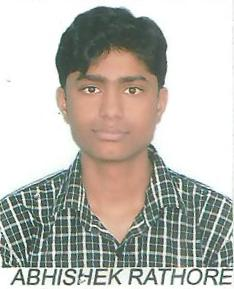
\includegraphics[scale=0.8]{Abhishek_Rathore_Photo.jpg}\\
\end{tabular}

\section*{Objective}
To seek challenging assignment and responsibility, with an opportunity for growth and career advancement as successful achievements.
\section*{Education}
\begin{tabular}{|l|l|l|l|l|}
\hline
Degree & College/School & University & Passing Year & Pass Percentage\\
\hline
B. Tech & JKIAPT & Allahabad University & 2017 & 72.04 (till 5th sem)\\
\hline
Intermediate & BDG SVM, Jhansi, UP & Uttar Pradesh Board & 2012 & 77.80\\
\hline
High School & BDG SVM, Jhansi, UP & Uttar Pradesh Board & 2010 & 82.67\\
\hline
\end{tabular}

\section*{Projects}
\begin{itemize}
\item[$\bullet$]\textbf{Hotel Guest Server Robot.}\\November 2015- March 2016\\Members: Gorji Parameswar Sampath, Aditya Kumar, Jatin Mittal.

A hotel wing is abstracted as an arena for this project. Guests indicate their service requests outside their doors. The Robot (ATmega 2560) is programmed to traverse this hotel wing (using White line, Sharp IR range, Proximity sensors) and look for service requests (using color sensor) and provide them in the order of priority. One of the services that the robot has to provide is removal of trash from the guests’ rooms (using mechanical arm).
\item[$\bullet$]\textbf{Website: Online FIR System}\\November 2015- January 2016

It enables Citizens to submit First Information Report against any crime in a very quick and easy way through internet and enables police department to get FIR’s in quick and systematic way.
\item[$\bullet$]\textbf{Caretaker Robot.}\\November 2014 - March 2015 \\Members: Gorji Parameswar Sampath, Aditya Kumar, Ratnesh Yadav.

This project was based on Atmega 2560, Xbee Modules, Camera, Image Processing using OpenCV and Python to deliver provisions to patients in a hospital.
\end{itemize}
\section*{Technical Skills}
\begin{itemize}
\item[$\cdot$]Programming Languages
\begin{enumerate}
\item C
\item Java
\item Python
\item Embedded C
\item SQL
\end{enumerate}
\item[$\cdot$]Tools and Technologies Used
\begin{enumerate}
\item J2SE
\item J2EE
\item Atmel Studio
\item OpenCV.
\end{enumerate}
\end{itemize}
\section*{Soft Skills}
\begin{itemize}
\item[$\cdot$] A Good Leader.
\item[$\cdot$] Team player.
\item[$\cdot$] Optimistic. 
\end{itemize}
\section*{Extra-Curricular Activities}
\begin{itemize}
\item[$\cdot$] Robotics Competition.
\item[$\cdot$] Google Code Jam.
\end{itemize}
\section*{Co-Curricular Activities}
\begin{itemize} 
\item[$\cdot$] Dancing.
\item[$\cdot$] Drama. 
\end{itemize}
\section*{Personal Details}
\begin{itemize}
\item[$\cdot$]Father's Name : Mr.Rajaram Rathore.
\item[$\cdot$]Mother's Name : Mrs. Kiran Rathore.
\item[$\cdot$]Sex           : Male.
\item[$\cdot$]Date of Birth : November 09, 1996.
\item[$\cdot$]Nationality   : Indian.
\item[$\cdot$]Martial Status: Single.
\end{itemize}
\section*{Declaration} I hereby declare that the above information is true and authentic to the best of my knowledge.
\section*{Date} May 27,2016.

\end{document}
